\chapter{Redefining the CMS Data Format}
\chaptermark{Redefining the CMS Data Format}
\thispagestyle{plain}  % First page has default style
\pagestyle{chapterpages}
\label{Section:Chapter5}
\minitoc

Within the CMS computing model, the \textbf{RAW} data format represents the full detector output and is the first available offline copy of an event following its acceptance by the HLT. It contains ``raw'' detector information, the L1 trigger result, the result of the HLT selections and other metadata.  The \textbf{RECO} format is derived from this complete record, and is the most CPU-intensive part of the CMS data processing chain because it involves reconstructing physics objects. This is followed by the \textbf{AOD} data format, a ``distilled" version of RECO designed to enable a broad range of physics analyses. Beyond AOD, CMS provides increasingly compact data formats, each offering different levels of information and precision.

The motivation to improve the RAW data format stems from the growing demands on the CMS data processing system. One of the primary challenges is the increasing complexity of events resulting from higher PU conditions. This complexity has a direct impact on the size of RAW events, imposing considerable strain on storage and bandwidth.  On average, RAW data currently occupies around $1.5\unit{MB}$ per event for pp collision data and approximately $2\unit{MB}$ per event for simulated events, with size expected to scale approximately linearly with PU. Therefore, it is necessary to explore improvements or data-reduction strategies for the RAW data format to prepare CMS for the higher PU conditions anticipated in future runs. 

This chapter will outline the main contributor to event size in the current RAW data format. This will be followed by the most recent data-reduction developments introduced in an alternative format, referred to as \textbf{RAW'}.

\section{Impact of the Silicon Strip Tracker on RAW size}
The \textbf{RAW} data format is constructed by collecting data fragments from all CMS subdetectors and assembling them into complete events. These fragments are read out by FEDs, which digitise the analogue signals and perform initial digital processing before passing the data to the event builder. Each subdetector is served by a number of FEDs, with the number depending on the its complexity and channel count.

The tracking subdetectors contribute the largest share of data to the RAW data format due to their exceptionally high channel density compared to other CMS subdetectors. In particular, the SST is the dominant contributor corresponding to roughly $\sim 50\%$ of the RAW event size because of the large number of FEDs dedicated to its readout. An overview of the number of channels and associated FEDs for all CMS subdetectors is provided in Table~\ref{Table:Chapter4_RAW_Channels_FED}.

\begin{table}[htbp]
\centering
\renewcommand{\arraystretch}{1.5} % Increase row height
\begin{tabular}{|l|c|c|}
\hline
Subdetector & Number of Channels & Number of FEDs \\
\hline \hline
Pixel tracker & $\sim124\unit{M}$ & 108 \\
\arrayrulecolor{lightgray} \hline
Strip tracker & $\sim9.3\unit{M}$ & 440 \\
\arrayrulecolor{lightgray} \hline
Preshower & $\sim144\unit{k}$ & 56 \\
\arrayrulecolor{lightgray} \hline
ECAL & $\sim75\unit{k}$ & 54 \\
\arrayrulecolor{lightgray} \hline
HCAL & $\sim9\unit{k}$ & 32 \\
\arrayrulecolor{lightgray} \hline
Muons CSC & $\sim500\unit{k}$ & 8 \\
\arrayrulecolor{lightgray} \hline
Muons RPC & $\sim192\unit{k}$ & 3 \\
\arrayrulecolor{lightgray} \hline
Muons DT & $\sim195\unit{k}$ & 10 \\
\arrayrulecolor{lightgray} \hline
\arrayrulecolor{black} \hline
\end{tabular}
\caption[CMS subdetector read-out parameters]{CMS subdetector read-out parameters. Values extracted from Ref.~\cite{LHC_CMS,CMS_Tracker_Phase1_Upgrade_2}.}
\label{Table:Chapter4_RAW_Channels_FED}
\end{table}

Given the significant contribution of the SST to the overall RAW event size, a promising strategy for data reduction is to optimise the information retained from the FED output. As discussed in Section~\ref{Section:Chapter4_Reconstruction_of_PF_elements}, clusters in the tracker are formed from contiguous strips with signal above predefined thresholds. For each cluster, the information stored in the RAW data includes the index of the first strip in the cluster and the ADC amplitudes for each strip within the cluster. Hence, exploring alternative representations of cluster information in the RAW data may offer additional opportunities for reducing the SST data volume.

\section{RAW' Data Format: Iteration 1}
\label{Section:Chapter5-RAW'_Iteration_1}
Reducing cluster-level information invites a key question: \textit{how much information can be discarded without compromising the accuracy of reconstructed physics observables?} To address this question, it is essential to consider the physical meaning encoded in the shape and structure of each cluster. 

A strip cluster represents a localised charge distribution induced by a charge particle traversing the subdetector. This distribution is typically non-uniform, exhibiting a peak where the maximum charge is deposited, along with signal tails extending over adjacent strips. Additionally, the particle's angle of incidence, entry point, and trajectory through the silicon sensor can introduce asymmetries in the charge distribution. The width of the cluster can also vary, with clusters associated with reconstructed tracks (on-track clusters) typically being narrower and more symmetric than those not linked to any track (off-track clusters).

Despite this complexity, the full cluster shape may not always be necessary to retain. It is therefore reasonable to consider whether a simplified, symmetric distribution could approximate the underlying charge profile while preserving the essential physics information. To evaluate the feasibility of such approximations, statistical measures such as skewness and kurtosis are used to characterise the shape of the cluster's charge distribution. These measurements are performed in different collision environments, including events with high jet activity, energetic isolated muons, and minimally biased pp collisions. Skewness values are typically close to zero or slightly positive ($\sim 0.23$), indicating only mild asymmetry. Additionally, kurtosis offers insight by quantifying the peakedness and tail behaviour of the distributions. In particular, Fisher kurtosis~\cite{Kurtosis}\footnote{The kurtosis of a standard normal distribution is three. Fisher kurtosis is a modified version of the standard Pearson kurtosis, normalising the Gaussian distribution to have a kurtosis of zero. This makes it easier to interpret deviations from normality: positive values indicate heavier tails (leptokurtic), and negative values indicate flatter distributions (platykurtic).} reveal that strip charge distributions are generally platykurtic, with values around -1.6. This is comparable to a uniform (rectangular) distribution, which has a Fisher kurtosis of -1.2.

These observations suggest that much of the cluster structure can be effectively summarised using a reduced set of parameters.  In the \textit{RAW'} data format, the per-strip ADC count (charge) is replaced with a \textit{simplified rectangular approximation} that preserves the original cluster width. The information stored per cluster consists of:

\begin{itemize}
    \item \textbf{Barycenter}: The charge-weighted centre of the cluster, serving as an approximation of the point at which the particle traversed the subdetector.
    \item \textbf{Width}: The number of strips forming the cluster.
    \item \textbf{Average charge}: The total charge (sum of ADC counts) in the cluster divided by the width of the cluster.
\end{itemize}

In the \textbf{RAW'} data format, the SST contribution to the event size is reduced to approximately 70\% of its original size. This corresponds to an overall event size reduction of approximately 20–25\% compared to the original \textbf{RAW} data format.

\subsection{Tracking performance}

While this new data format provides a significant reduction in the SST data volume, its viability ultimately depends on whether it preserves the physics performance necessary for CMS analyses. Therefore, it is essential to verify that this reduced cluster representation does not degrade the quality of track reconstruction. This can be assessed through the \textit{tracking efficiency}, defined as the fraction of simulated particles successfully reconstructed. The tracking performance of the RAW' data format is shown in Fig.~\ref{Figure:Chapter5_TrackingPerformance_1}, where comparisons of tracking efficiency as a function of $p_\mathrm{T}$ and $\phi$ are presented relative to the standard RAW format.

\begin{figure}[h]
        \centering
        % First row
        \begin{subfigure}[b]{0.49\textwidth}
            \centering
            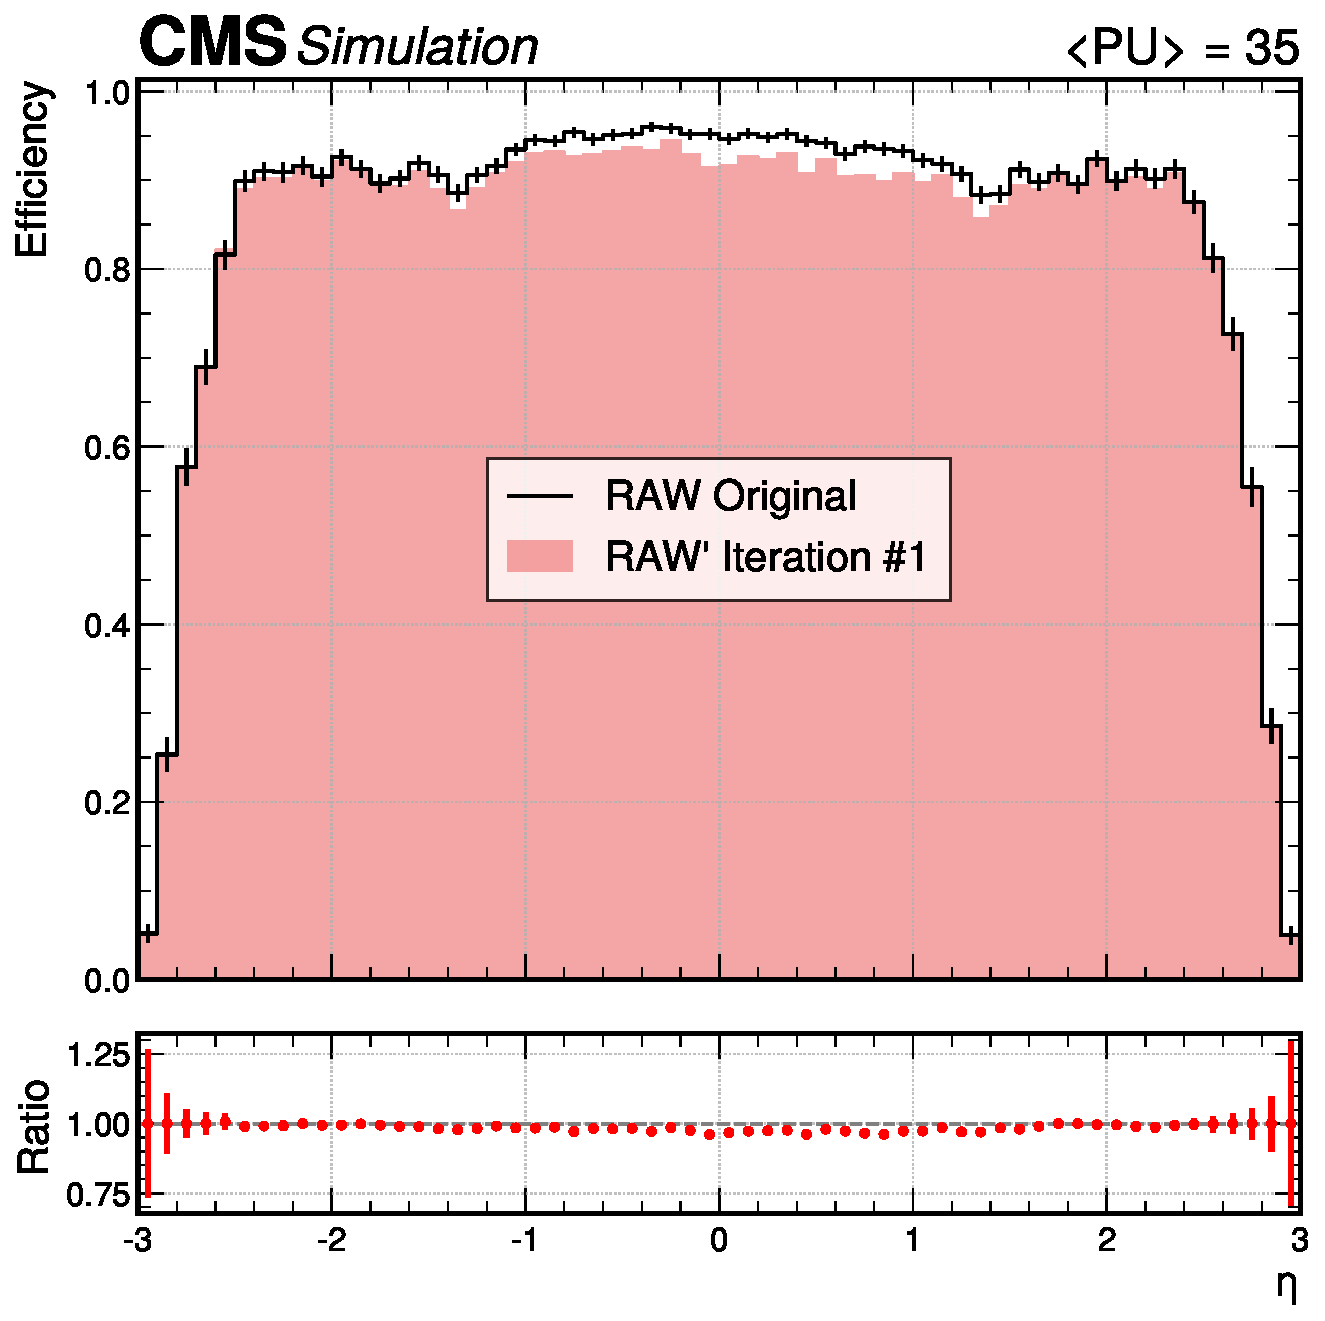
\includegraphics[width=\textwidth]{Figures/Chapter5/efficiency_comparison_1_eta.pdf}
            \caption{}
        \end{subfigure}
        \begin{subfigure}[b]{0.49\textwidth}
            \centering
            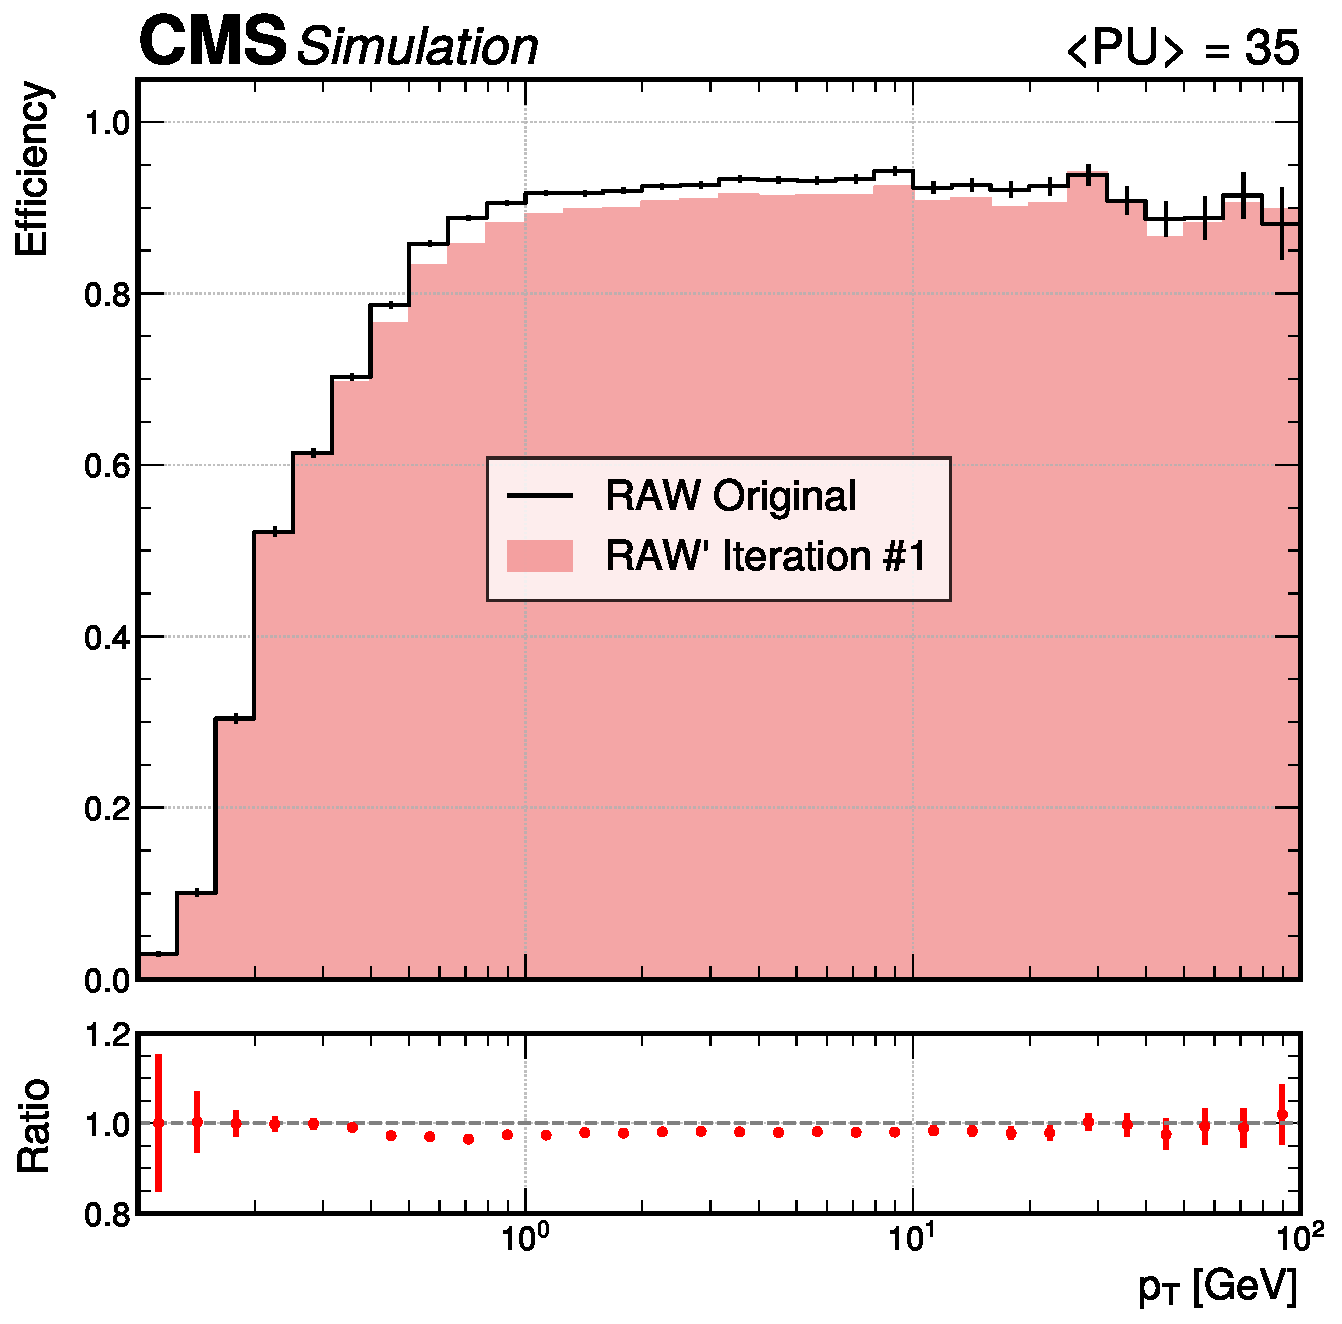
\includegraphics[width=\textwidth]{Figures/Chapter5/efficiency_comparison_1_pt.pdf}
            \caption{}
        \end{subfigure}
    \caption[Comparison of the track reconstruction efficiency as a function of $\eta$ and $p_\mathrm{T}$ between the original RAW format and the first iteration of RAW'.]{Comparison of the track reconstruction efficiency as a function of \textbf{(a)} $\eta$ and \textbf{(b)} $p_\mathrm{T}$ between the original RAW format and the first iteration of RAW'. Results are based on simulated $t\bar{t}$ events.} 
    \label{Figure:Chapter5_TrackingPerformance_1}
\end{figure}

The tracking performance of the RAW' format appears promising, showing a small degradation in efficiency across both $\phi$ and $p_\mathrm{T}$, typically of the order of a few percent. However, it is also important to ensure that this also holds for the efficiency as a function of the vertex radius, as this directly impacts the reconstruction of displaced tracks. As shown in Fig.~\ref{Figure:Chapter5_TrackingPerformance_vertexPos_1}, there is a notable decrease in performance beyond a radius of approximately $10\unit{cm}$, with the efficiency becoming severely degraded above $20\unit{cm}$. 

\begin{figure}[h]
\centering
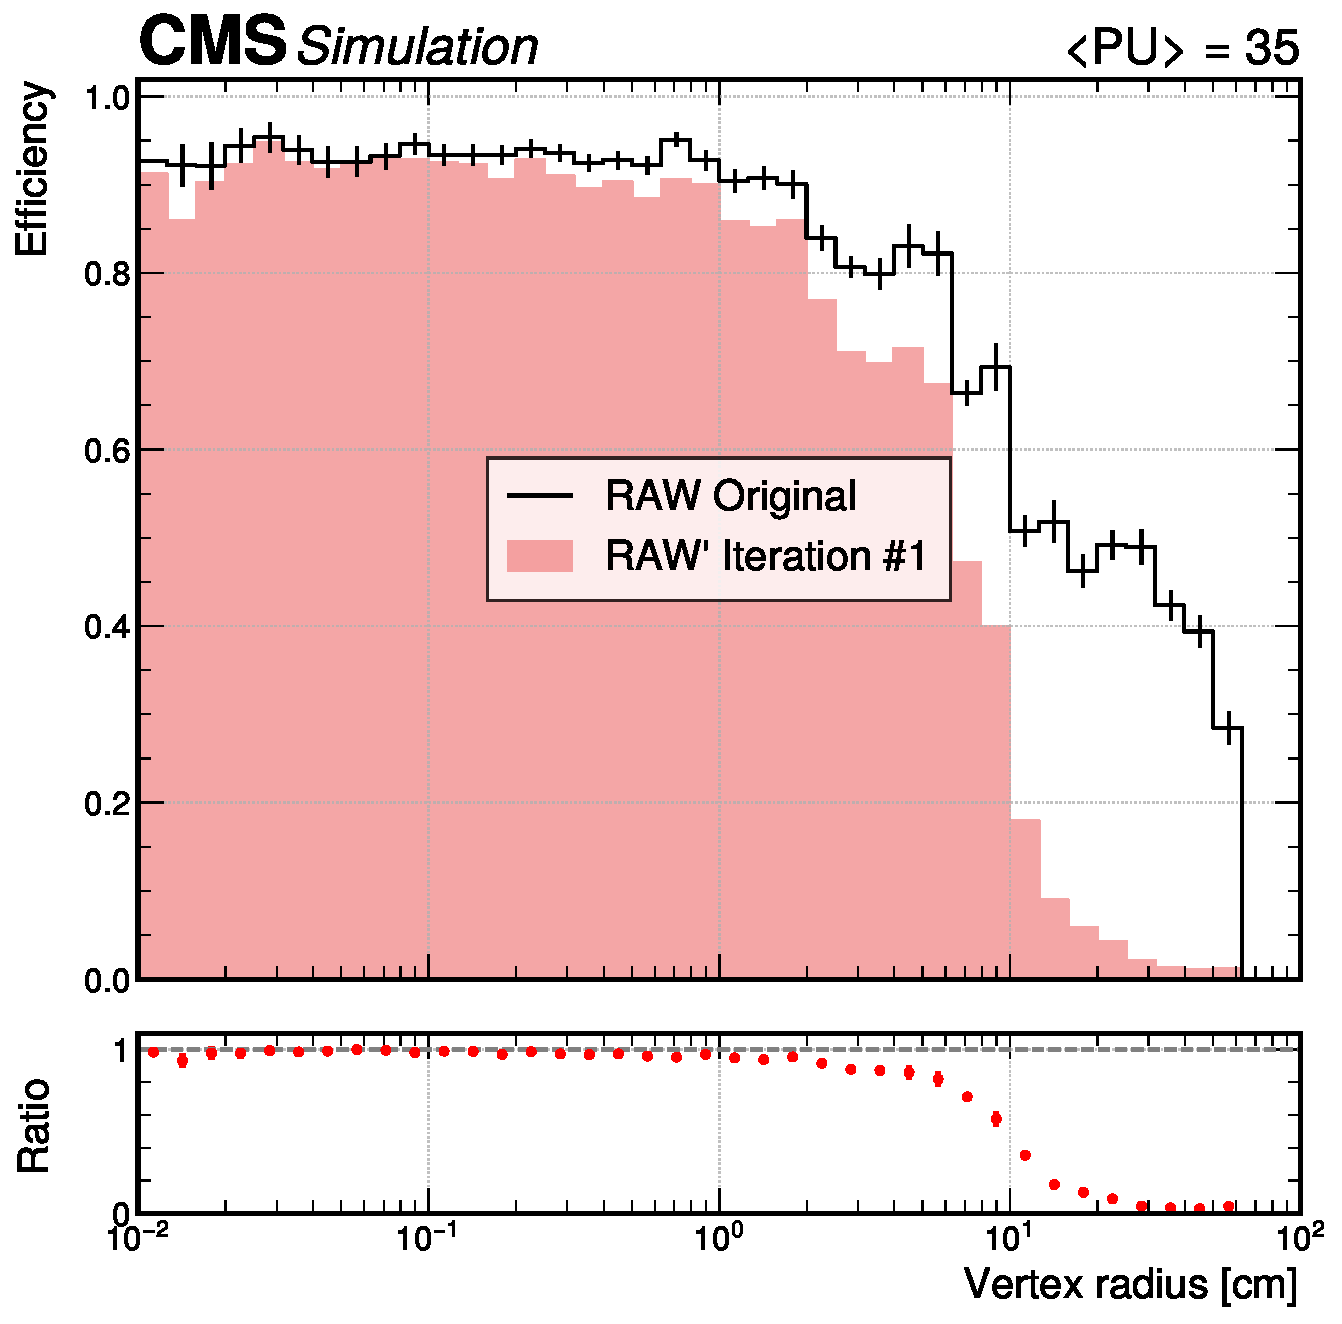
\includegraphics[width=0.8\textwidth]{Figures/Chapter5/efficiency_comparison_1_vertpos.pdf}
\caption[Comparison of the track reconstruction efficiency as a function of the vertex radius between the original RAW format and the first iteration of RAW'.]{Comparison of the track reconstruction efficiency as a function of the vertex radius between the original RAW format and the first iteration of RAW'. Results are based on simulated $t\bar{t}$ events.} 
\label{Figure:Chapter5_TrackingPerformance_vertexPos_1}
\end{figure}

To understand the observed degradation for displaced vertices, Table~\ref{Table:Chapter4_IterativeTrackingSeeds} provides insight into which iterative tracking steps are specifically designed to target such tracks. In particular, the \textit{MixedTriplet}, \textit{PixelLess}, and \textit{TobTec} steps are responsible for reconstructing displaced tracks. By examining the tracking efficiency broken down by iteration step (see Fig.~\ref{Figure:Chapter5_TrackingPerformance_bystep}), it becomes evident that the loss in efficiency at larger radii is primarily due to reduced performance in the PixelLess and TobTec steps.

\begin{figure}[h]
\centering
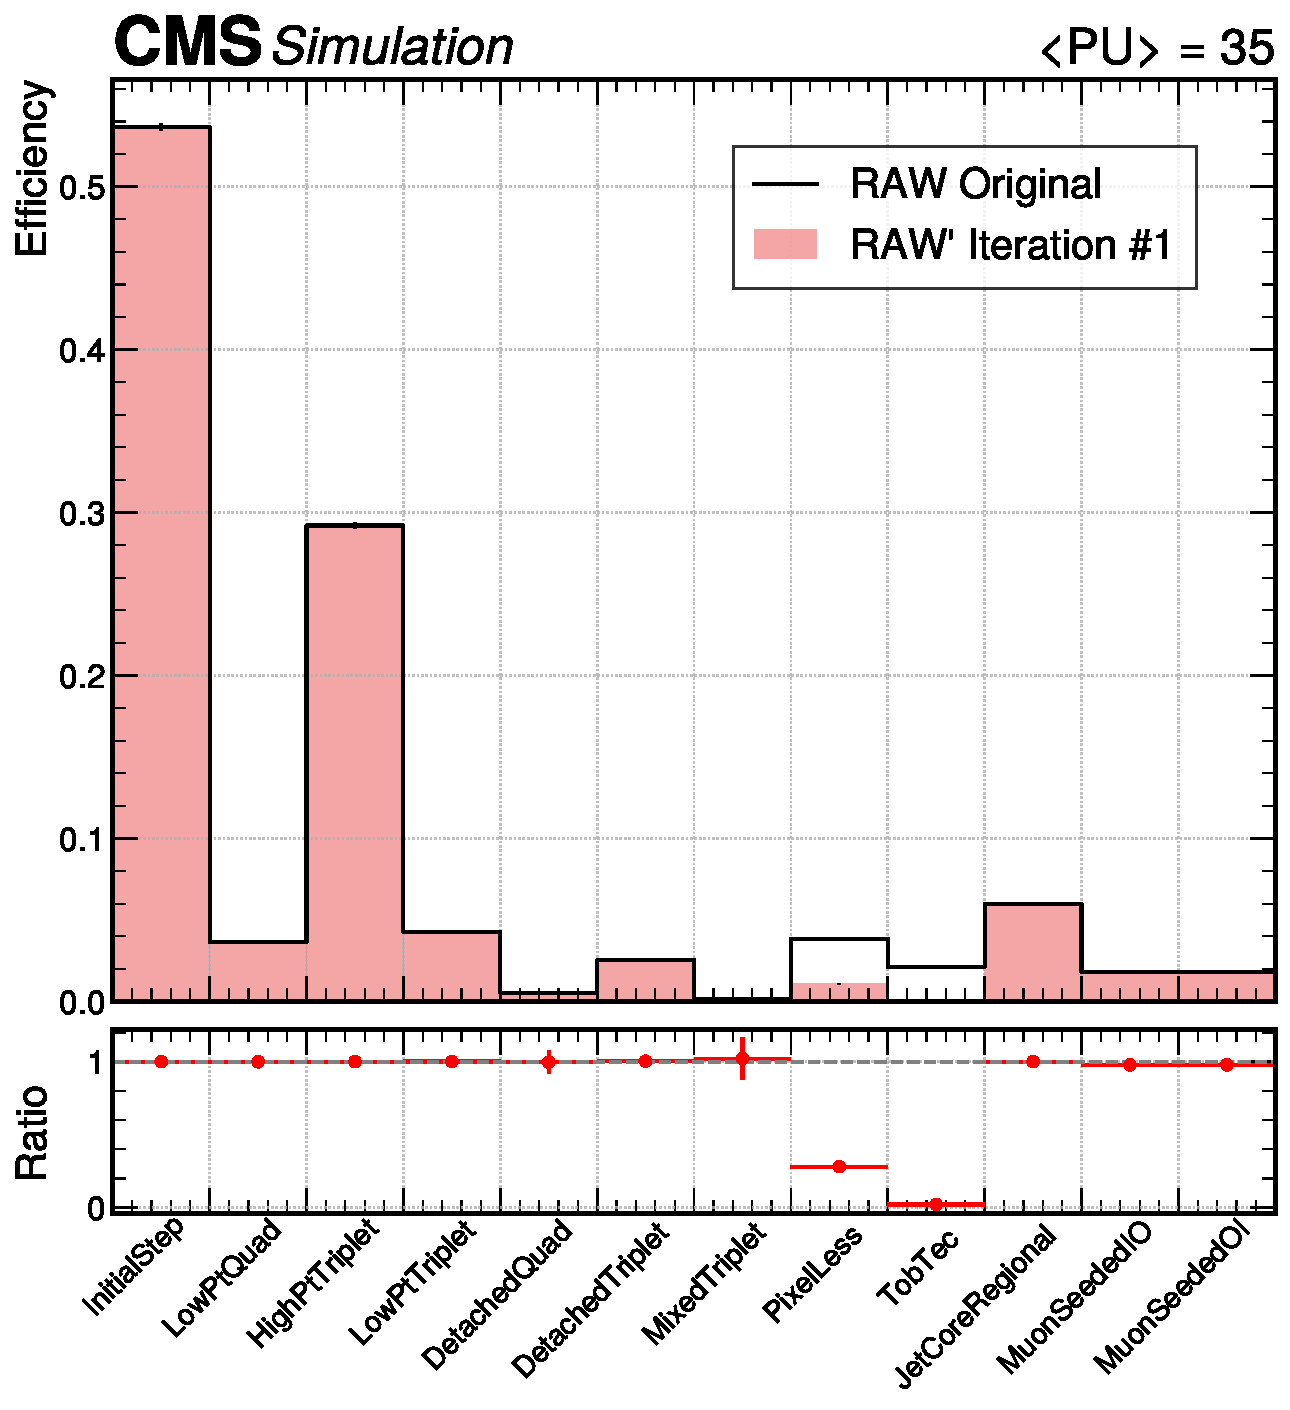
\includegraphics[width=0.8\textwidth]{Figures/Chapter5/efficiency_with_ratio.pdf}
\caption[Track reconstruction efficiency for the different iterations of the CMS iterative tracking algorithm.]{Track reconstruction efficiency for the different iterations of the CMS iterative tracking algorithm. Results are based on simulated $t\bar{t}$ events.}
\label{Figure:Chapter5_TrackingPerformance_bystep}
\end{figure}

\subsection{Complications from cluster shape approximation}

The observed inefficiency in the \textit{PixelLess} and \textit{TobTec} iterations is attributed to the use of cluster shape filters within the CMS iterative tracking algorithm. These filters are particularly effective in the high-combinatorial environment of the CMS tracker, where they help suppress the rate of misreconstructed tracks. However, the rectangular approximation of the cluster charge distribution in RAW' effectively removes the characteristic peaks and tails essential for shape-based discrimination.

One of the first checks performed by the cluster shape filters targets \textbf{saturated strips}. A cluster is flagged as saturated if it contains three consecutive strips with ADC counts above a predefined threshold. However, in this format, only the average cluster charge is stored, rather than the individual strip charges. This approximation can lead to incorrect filter outcomes. For example, if a single strip is sufficiently saturated, this can artificially elevate the average charge of the entire cluster above the saturation threshold, leading to a false positive from the filter. Conversely, clusters that genuinely meet the saturation condition may fail the filter if the average charge falls below the threshold due to dilution from strips with low ADC counts, resulting in a false negative. In comparison to the original format, approximately 99\% of saturated clusters fail this check.

An additional check performed is known as \textbf{trimming}. This step evaluates the presence of tails in the cluster's charge distribution by comparing the charge of each strip to that of neighbouring strips.  This check targets and removes clusters with disproportionately large tails. However, as only the average charge is stored, this filter is rendered ineffective, leading to clusters that would otherwise be rejected being falsely retained. 

Another important check is the presence of a \textbf{peak} in the cluster charge distribution. This step assesses whether the cluster exhibits a clearly defined local maximum. However, there is no local charge variation in this format, causing the filter to fail in detecting a peak within the flat distribution.

\section{RAW' Data Format: Iteration 2}

Motivated by the shortcomings of the initial RAW' format, particularly its inability to retain acceptable track reconstruction efficiency for displaced vertices, a second iteration has been developed. This updated format is specifically designed to address the limitations imposed by cluster shape-based filtering.

The original format of RAW' discussed in Section~\ref{Section:Chapter5-RAW'_Iteration_1} is retained, but a set of additional features is introduced to restore compatibility with cluster shape-based filtering. For the saturated strip check, the solution is straightforward. A boolean flag indicating saturation is computed from the original clusters and stored alongside the barycenter, width and average charge of the cluster. However, the trimming and peak-finding filters are more complex to replicate. This is primarily due to the timing and dependencies of their application within the reconstruction workflow. While the saturated strip check can rely on the original cluster, since the approximated rectangular clusters are constructed directly from it, the trimming and peak-finding filters are applied after cluster construction. At this stage, the original cluster is no longer available. Consequently, these filters cannot ``borrow'' information from the original strip-level data.

In particular, trimming and peak-finding require the estimated position and direction of a track as it passes through a specific detector layer, referred to as trajectory state on surface (TSOS). These quantities are only available once a track has been reconstructed, and cluster construction occurs earlier in the reconstruction chain. Therefore, TSOS-related inputs cannot be computed directly at that stage because no trajectory information exists. As a result, applying these checks during or immediately after clustering would require these track-dependent variables to be approximated or inferred through alternative means.

To address these challenges, the clustering step has been enhanced to incorporate additional information such as the beamspot position, tracker geometry, and noise conditions. With this additional input, basic versions of the trimming and peak filters can now be applied directly during cluster construction. The cluster’s position is estimated using its barycenter, and a vector from the beamspot is used to approximate the track direction toward the cluster. While the use of geometric and noise-related information introduces added complexity, particularly due to local-to-global coordinate transformations, the core structure of the RAW' format remains unchanged. The only addition is a single boolean flag that captures the combined outcome of the saturation, trimming, and peak filters. Despite this extension, the format still achieves a 20\% reduction in data size compared to the original.

\subsection{Tracking performance}

The central question for this updated RAW' format is whether it can recover the tracking inefficiencies introduced by the first version, particularly in reconstructing displaced tracks. Fig.~\ref{Figure:Chapter5_TrackingPerformance_2} shows the tracking efficiency as a function of $p_\mathrm{T}$, $\eta$, and vertex radius. While the first iteration already preserved efficiency reasonably well in $p_\mathrm{T}$ and $\eta$, leaving limited room for improvement, a significant recovery is observed in the vertex radius distribution. The inefficiencies at large displacements, where performance was most severely degraded, are substantially mitigated in this second iteration, demonstrating the effectiveness of reintroducing shape-based filtering logic.

\begin{figure}[h]
        \centering
        % First row
        \begin{subfigure}[b]{0.49\textwidth}
            \centering
            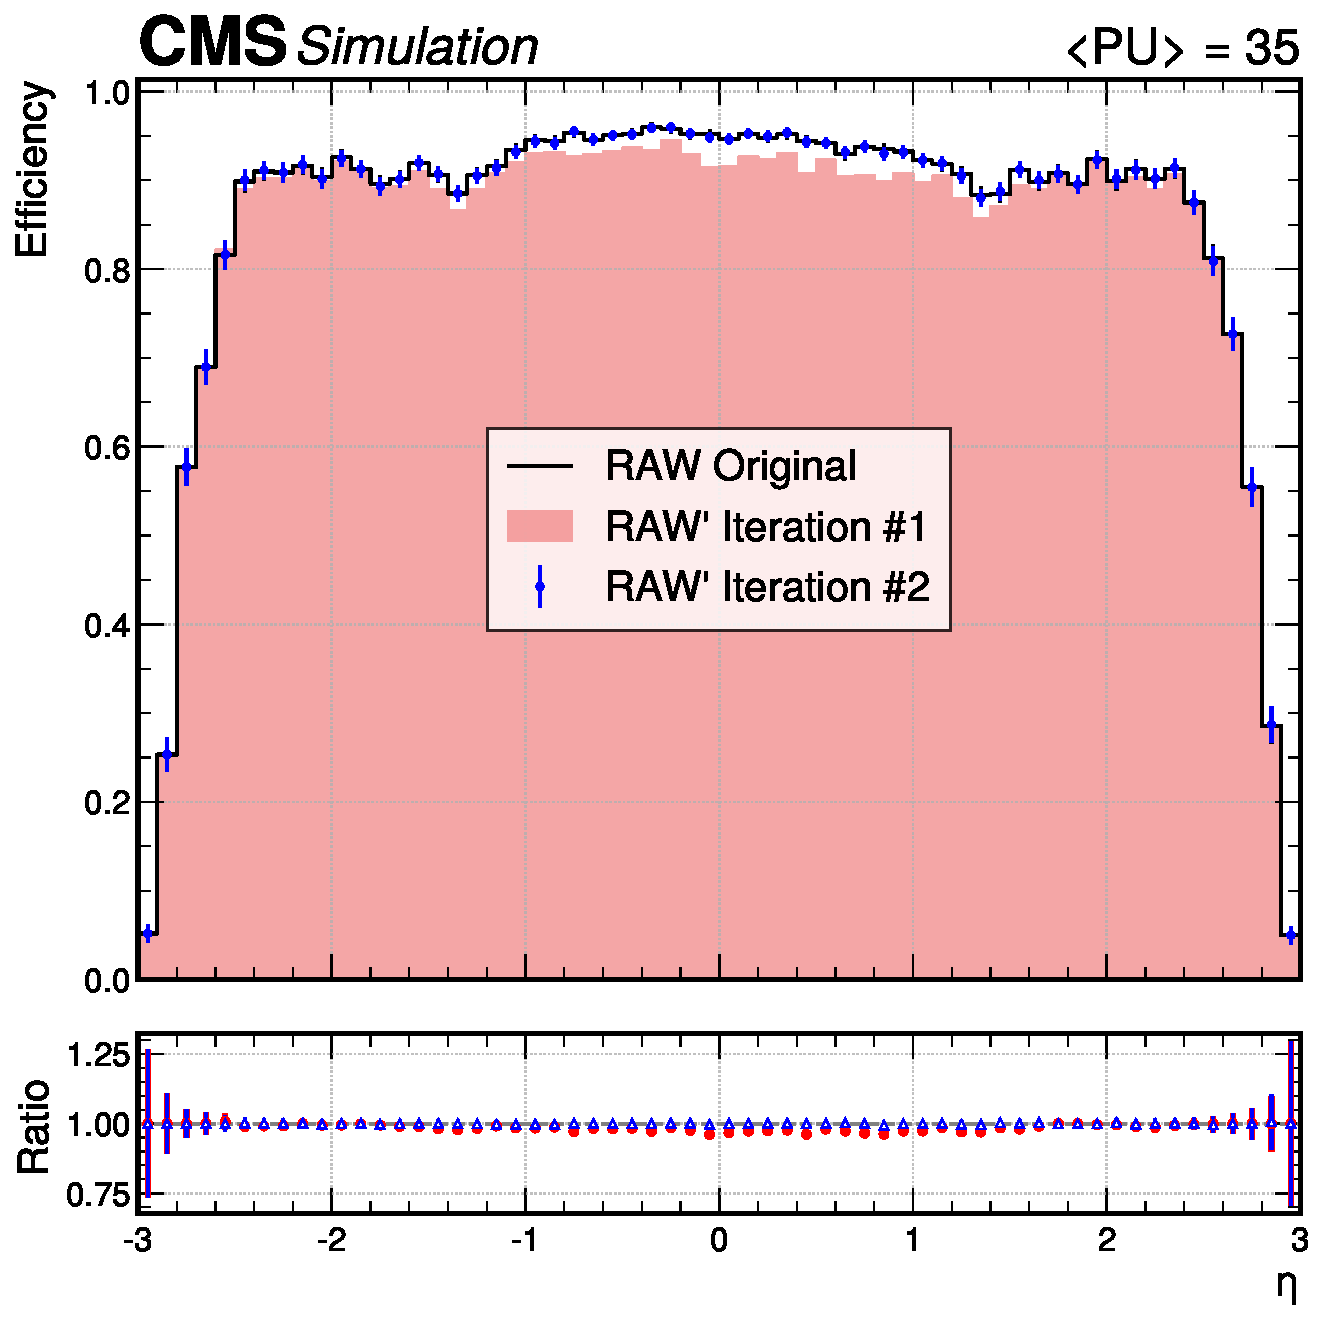
\includegraphics[width=\textwidth]{Figures/Chapter5/efficiency_comparison_2_eta.pdf}
            \caption{}
        \end{subfigure}
        \begin{subfigure}[b]{0.49\textwidth}
            \centering
            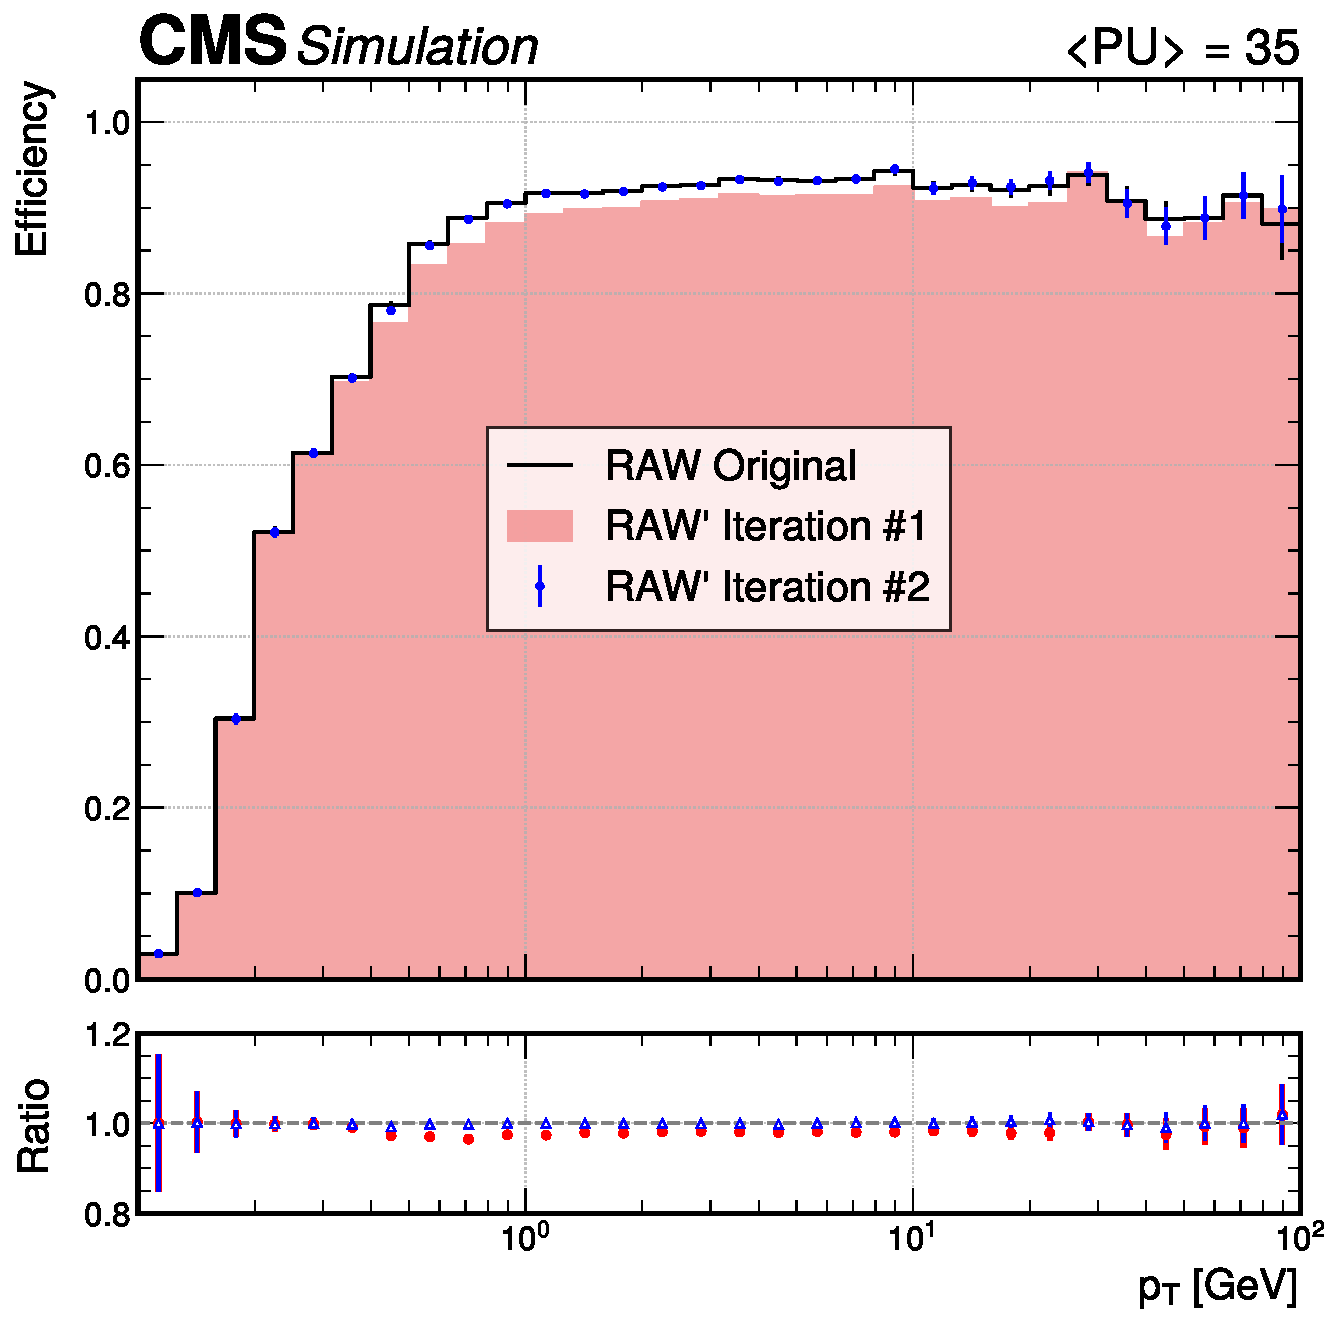
\includegraphics[width=\textwidth]{Figures/Chapter5/efficiency_comparison_2_pt.pdf}
            \caption{}
        \end{subfigure}

        \vspace{0.5cm}

        \begin{subfigure}{0.49\textwidth}
            \centering
            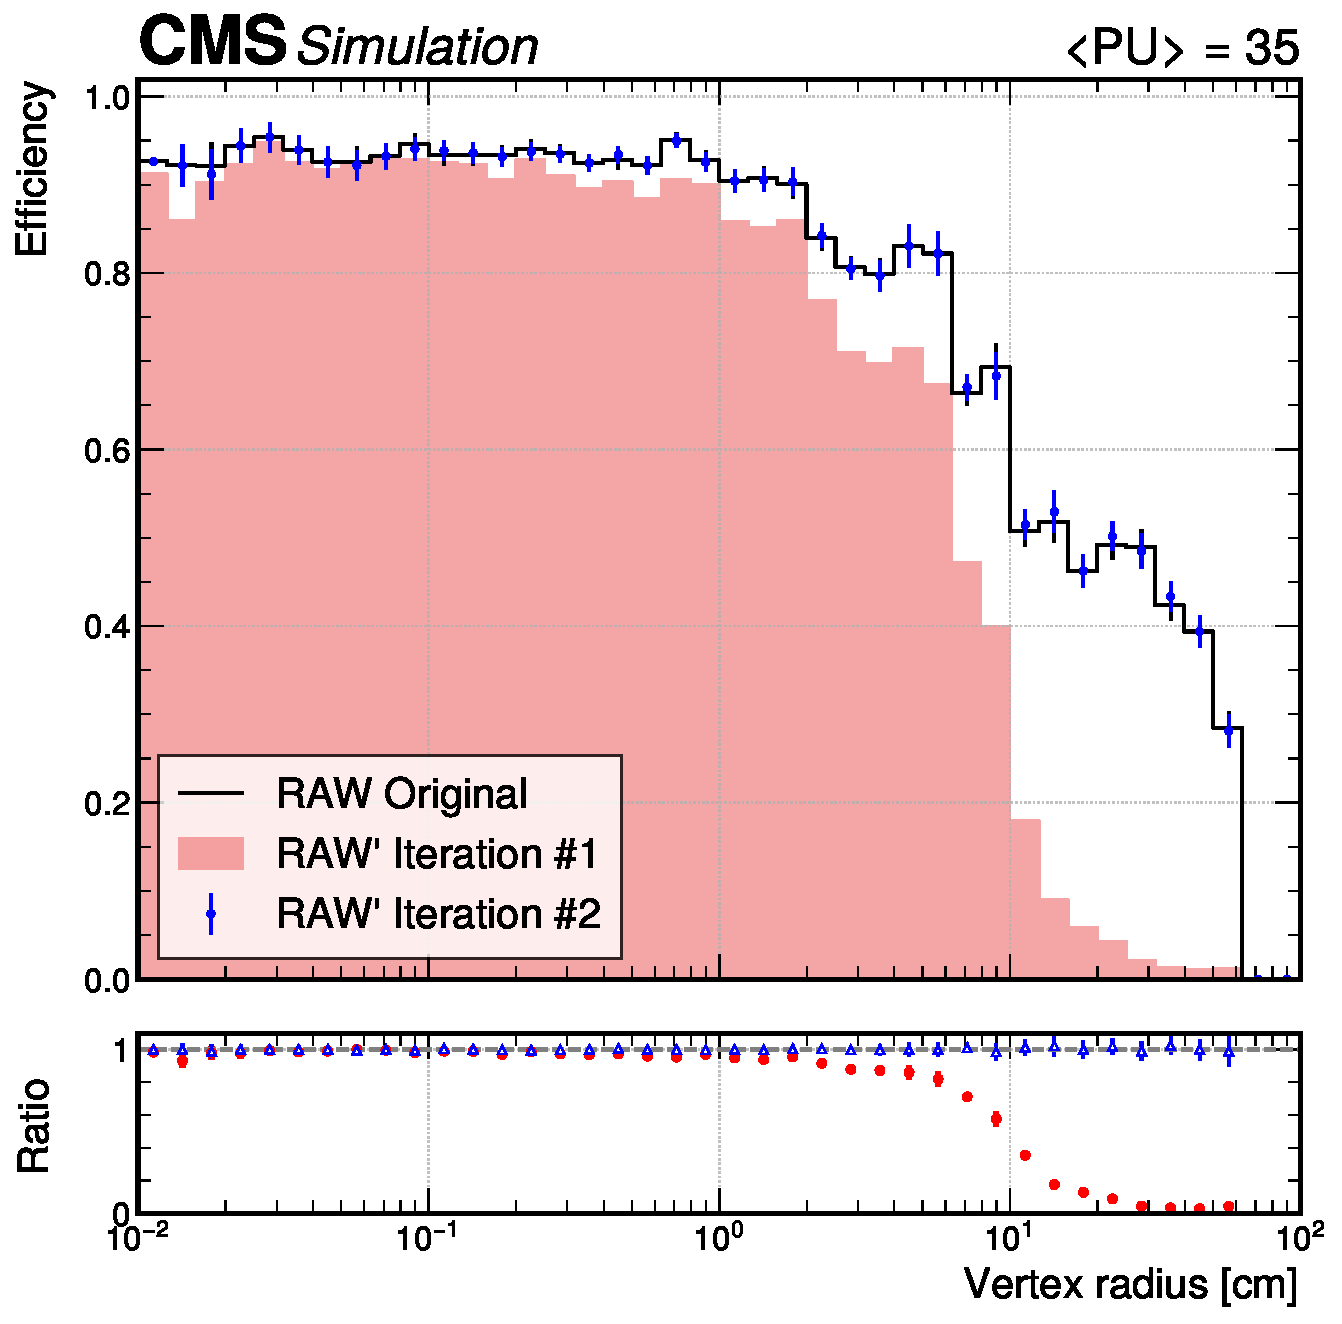
\includegraphics[width=\textwidth]{Figures/Chapter5/efficiency_comparison_2_vertpos.pdf}
            \caption{}
        \end{subfigure}
    \caption[Comparison of the track reconstruction efficiency as a function of $\eta$ and $p_\mathrm{T}$ between the original RAW format, and the alternative RAW' definitions.]{Comparison of the track reconstruction efficiency as a function of \textbf{(a)} $\eta$ and \textbf{(b)} $p_\mathrm{T}$ between the original RAW format, and the alternative RAW' definitions. Results are based on simulated $t\bar{t}$ events.} 
    \label{Figure:Chapter5_TrackingPerformance_2}
\end{figure}

In addition to these global metrics, tracking performance can be further evaluated by
examining the \textit{resolution} of reconstructed quantities such as the IP projections in the transverse plane ($d_{xy}$) and along the beam axis ($d_z$). Comparisons between the different data formats are presented in Figure~\ref{Figure:Chapter5_ResolutionComparison}.

\begin{figure}[h]
        \centering
        % First row
        \begin{subfigure}[b]{0.49\textwidth}
            \centering
            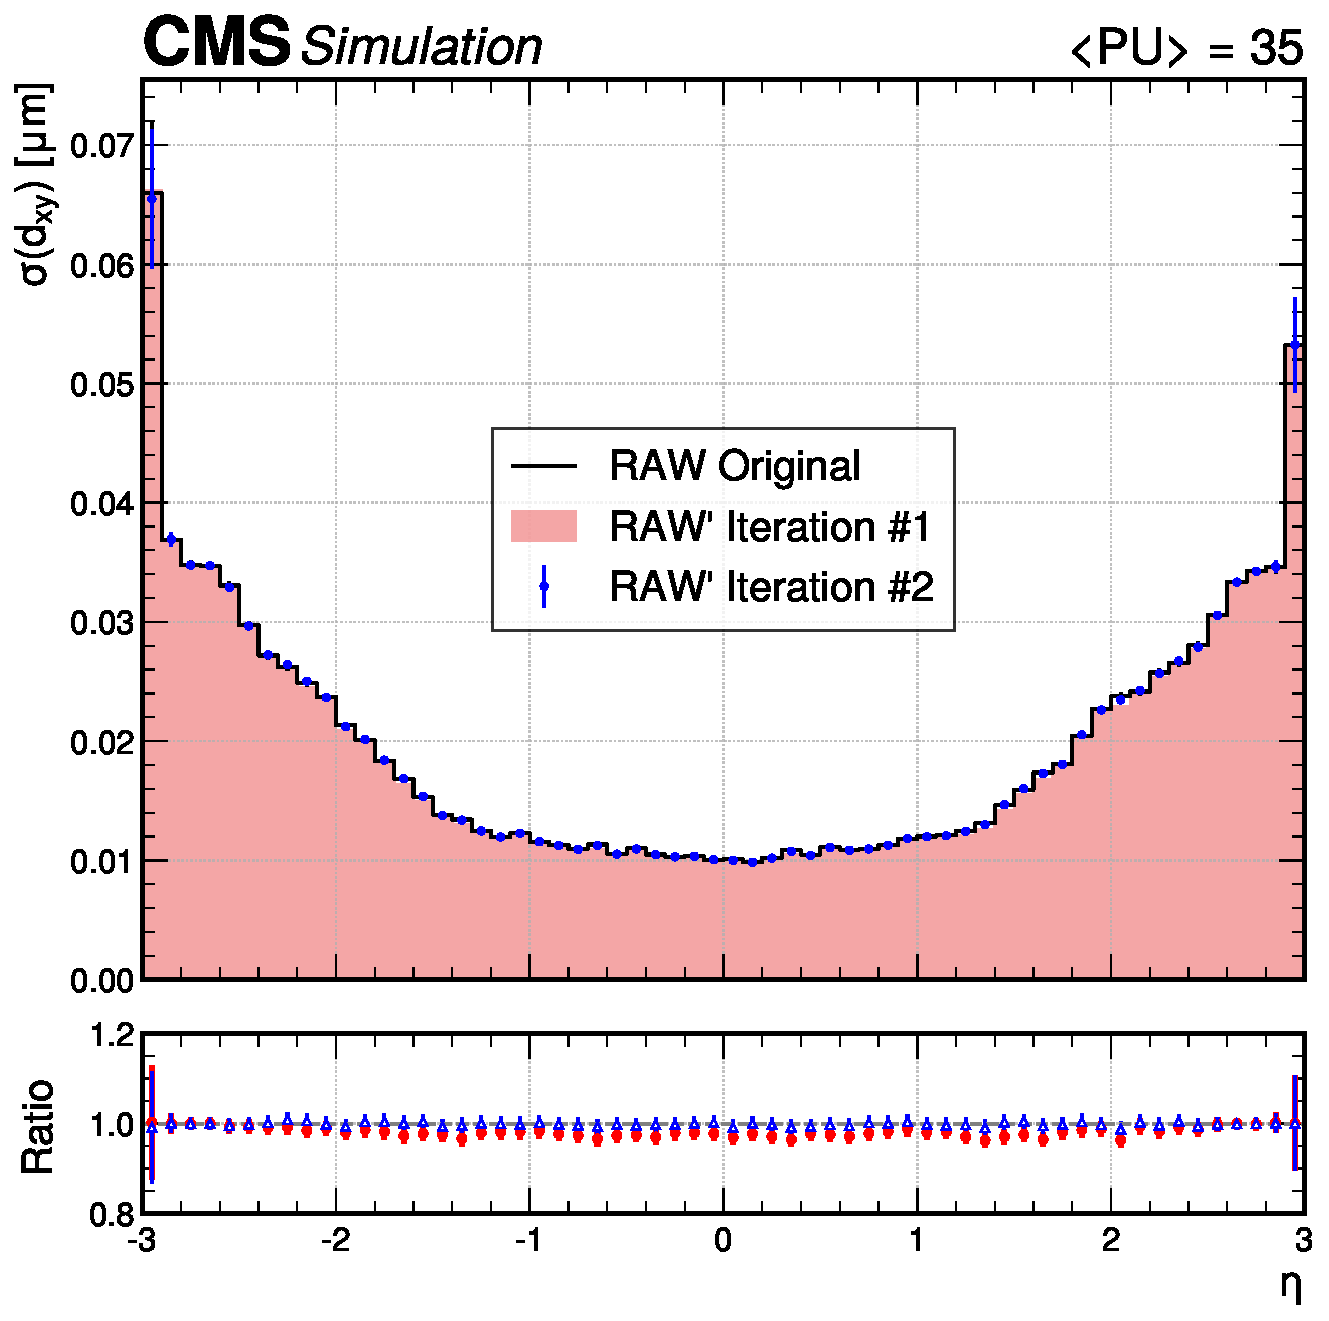
\includegraphics[width=\textwidth]{Figures/Chapter5/resolution_comparison_dxy_eta.pdf}
            \caption{}
        \end{subfigure}
        \begin{subfigure}[b]{0.49\textwidth}
            \centering
            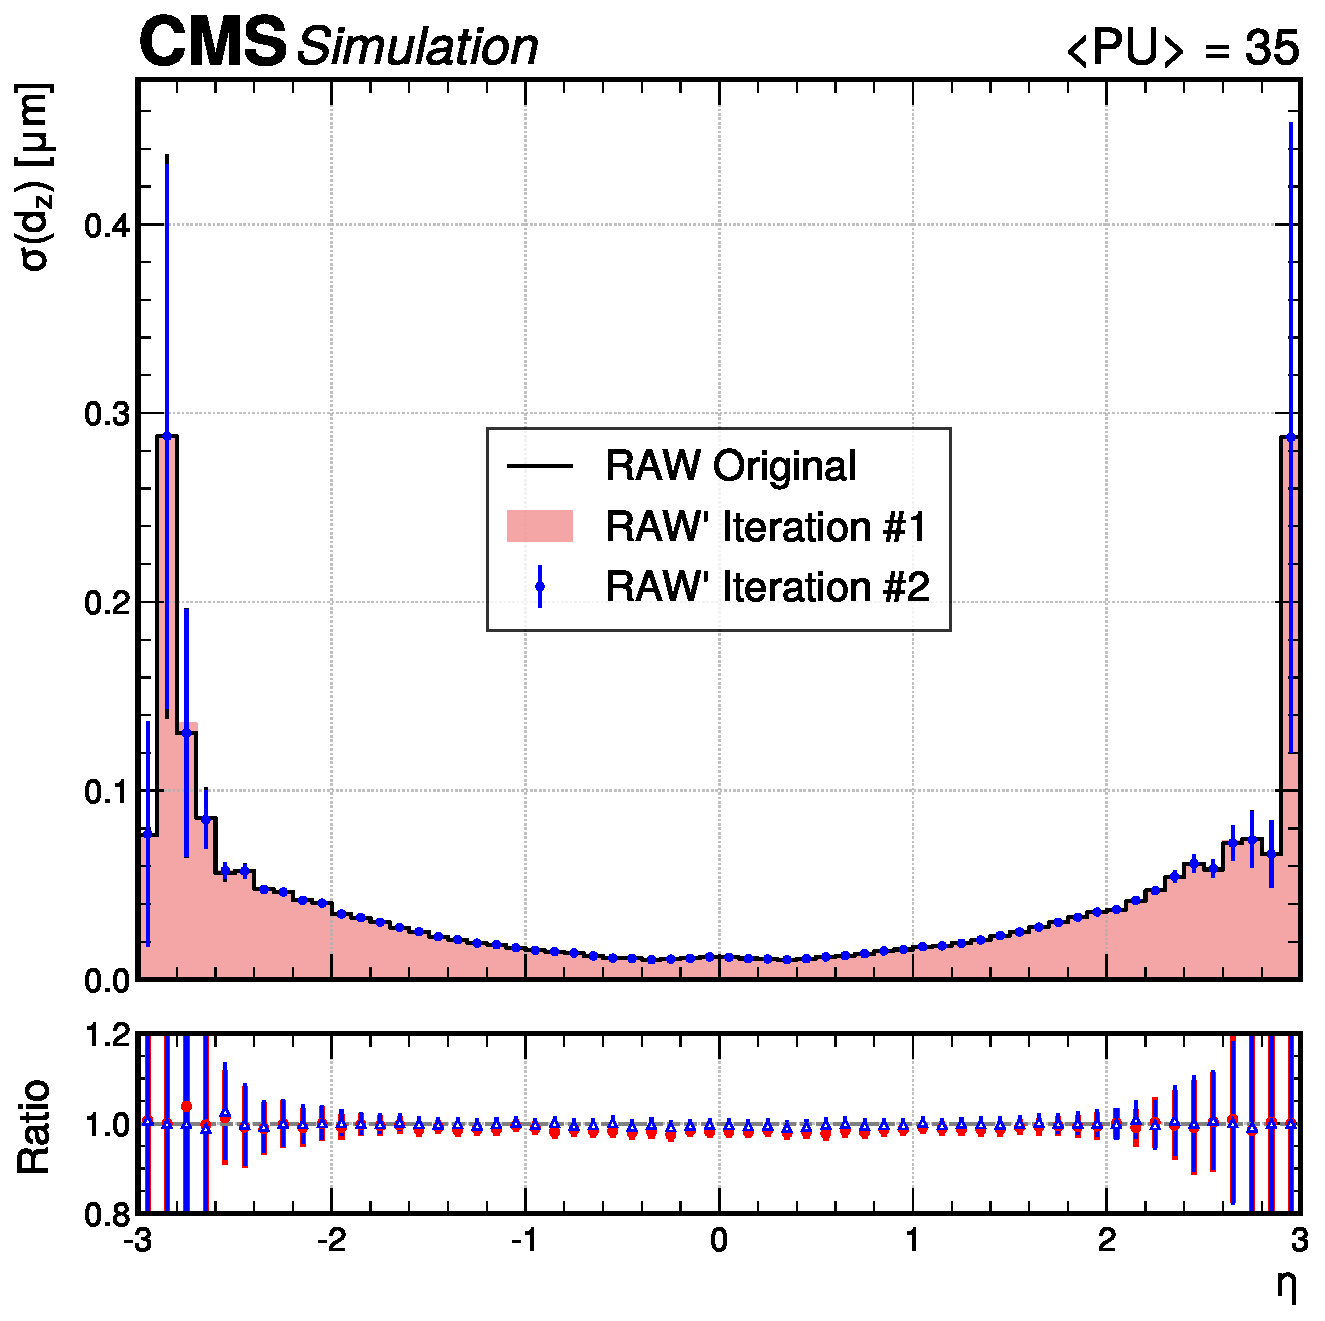
\includegraphics[width=\textwidth]{Figures/Chapter5/resolution_comparison_dz_eta.pdf}
            \caption{}
        \end{subfigure}
        
    \caption[Resolution of IP projections vs $\eta$ for RAW and RAW']{Comparison of the resolution of the \textbf{(a)} transverse and \textbf{(b)} longitudinal impact parameter (IP) projections as a function of $\eta$, comparing the original RAW format to the alternative RAW' definitions. Results are based on simulated $t\bar{t}$ events.}
    \label{Figure:Chapter5_ResolutionComparison}

    \label{Figure:Chapter5_ResolutionComparison}
\end{figure}

While the tracking efficiencies and resolutions achieved with the alternative RAW' format are promising, it is equally important to assess its impact on the reconstruction of long-lived particles with displaced decay signatures, such as the $\mathrm{K}_\mathrm{S}^0$ meson ($c\tau = 2.68\,\unit{cm}$)~\cite{ParticleMasses}. Key performance metrics include the number of reconstructed $\mathrm{K}_\mathrm{S}^0$ candidates and the transverse distance between the particle’s decay point and the primary vertex ($L_{xy}$). As shown in Fig.~\ref{Figure:Chapter5_KsReconstruction}, the updated format exhibits a significant improvement over the first RAW' iteration and achieves performance comparable to the original format. These results further highlight the effectiveness of the enhancements in restoring displaced tracking capabilities.

\begin{figure}[h]
        \centering
        % First row
        \begin{subfigure}[b]{0.49\textwidth}
            \centering
            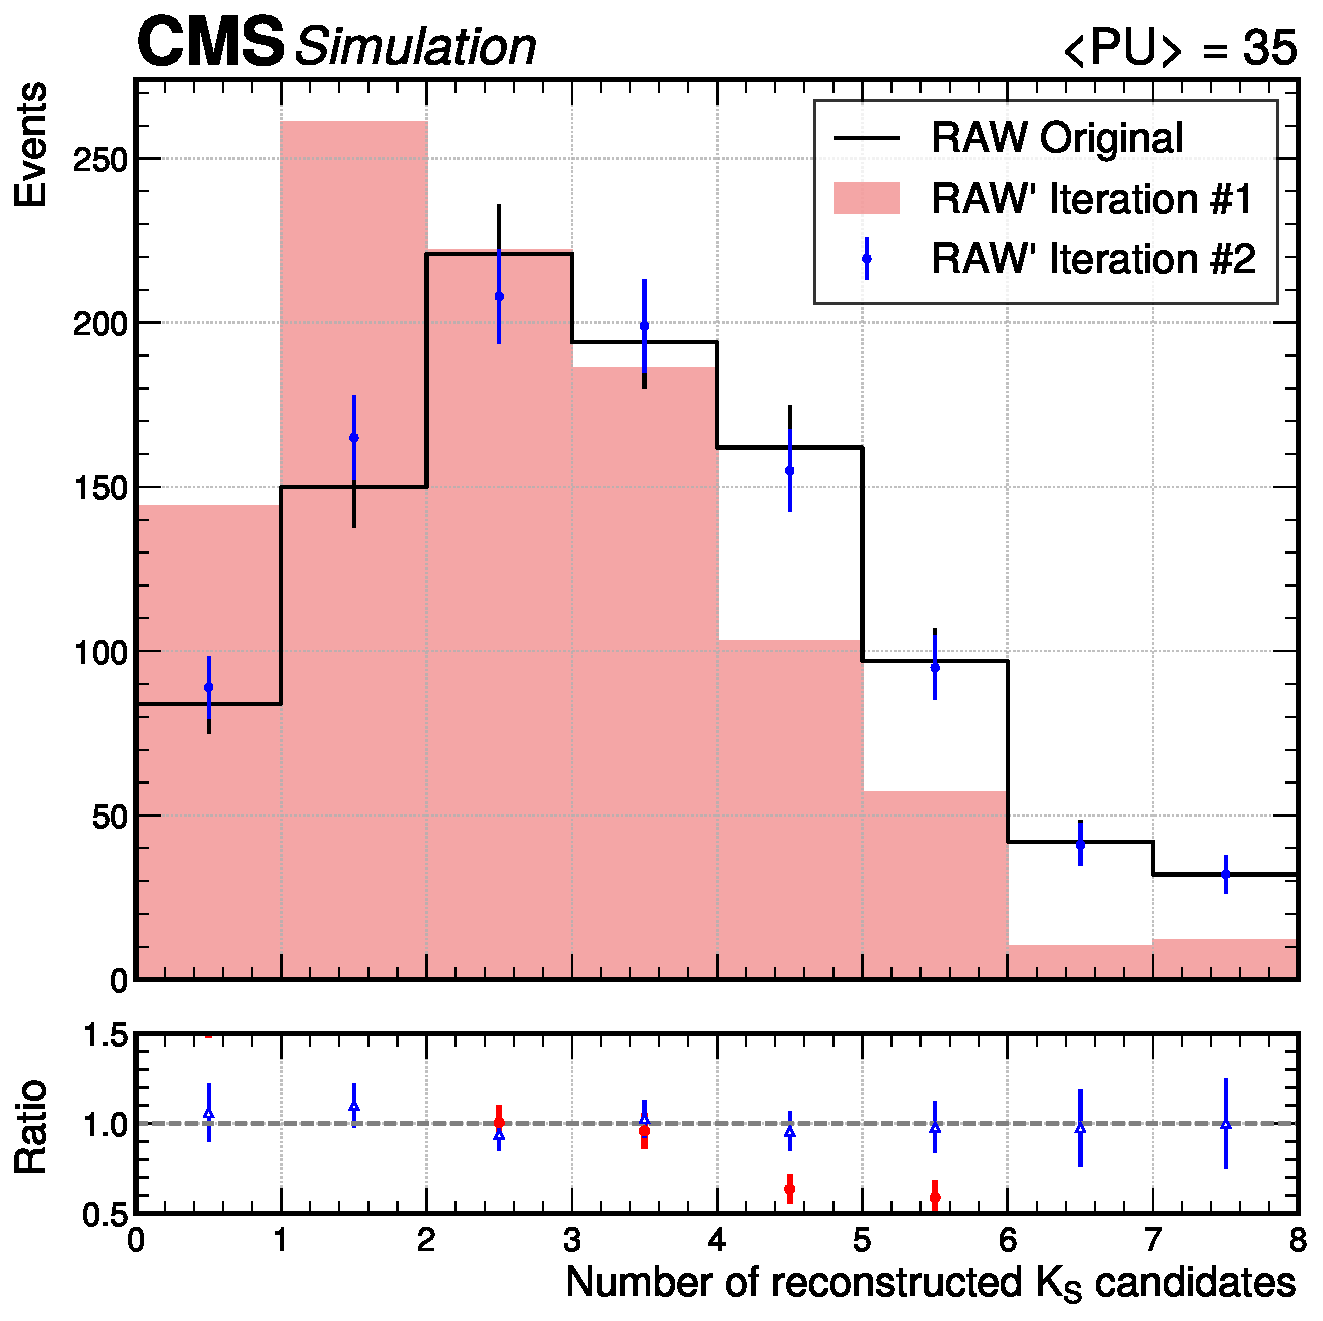
\includegraphics[width=\textwidth]{Figures/Chapter5/Ks_N.pdf}
            \caption{}
        \end{subfigure}
        \begin{subfigure}[b]{0.49\textwidth}
            \centering
            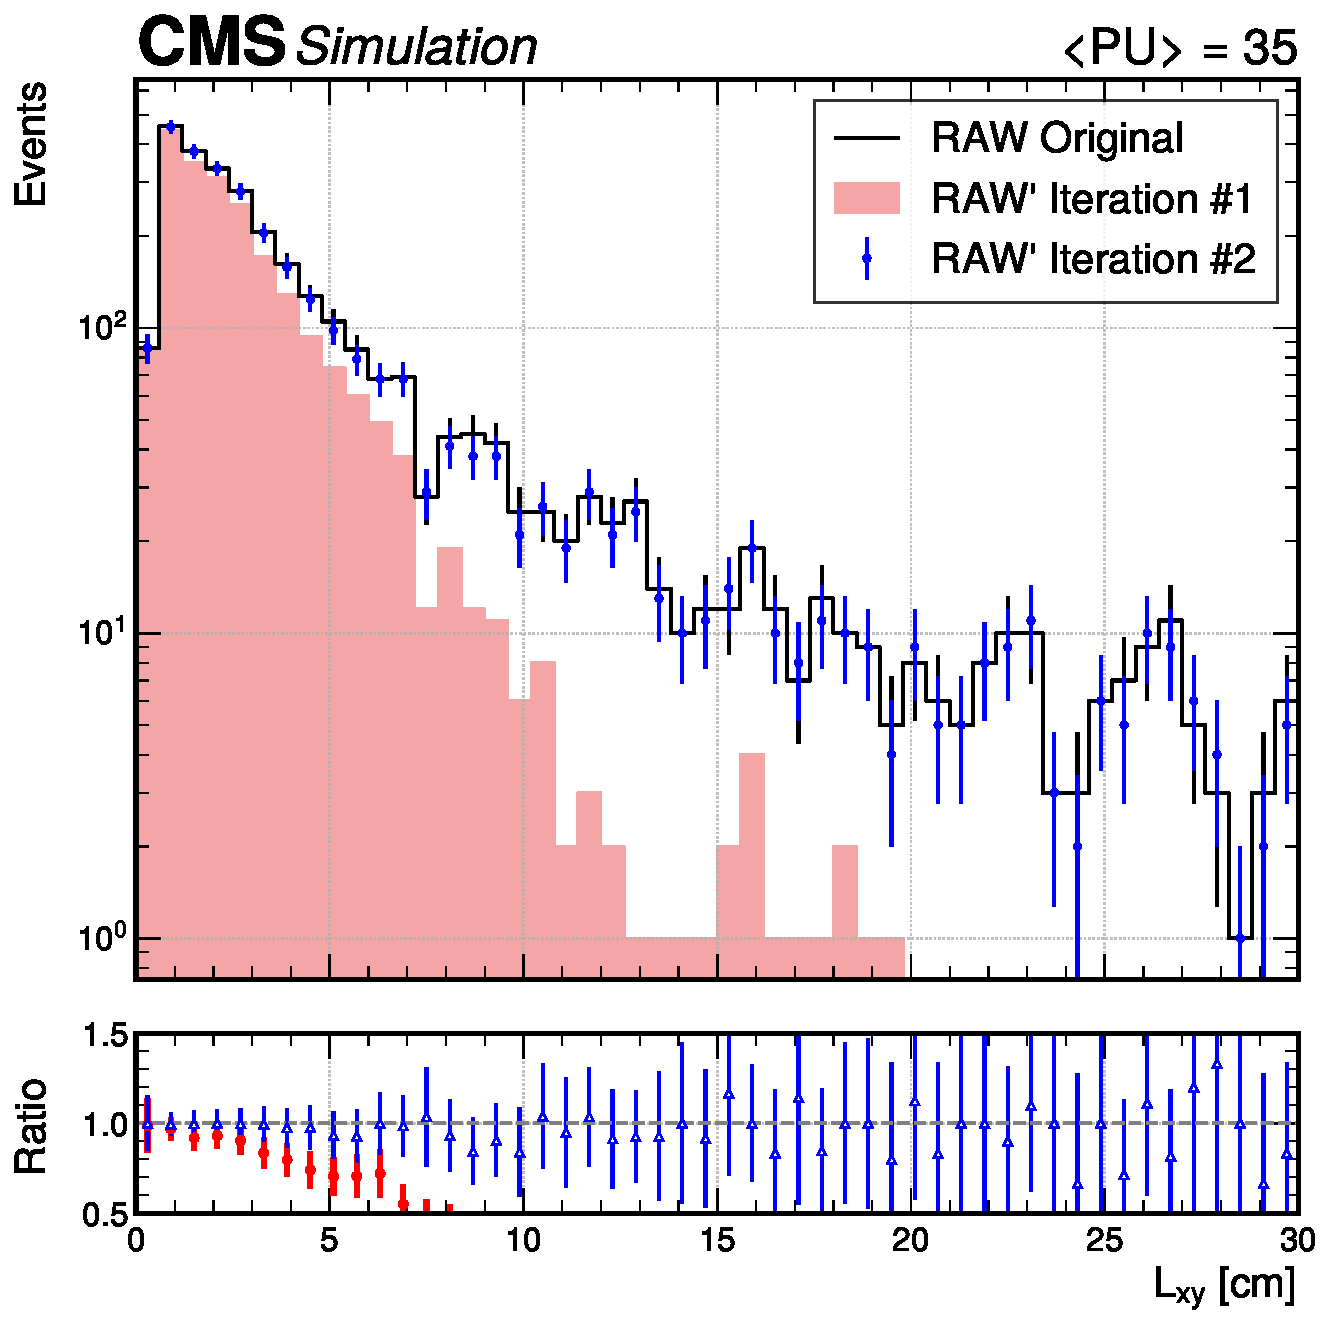
\includegraphics[width=\textwidth]{Figures/Chapter5/Ks_Lxy.pdf}
            \caption{}
        \end{subfigure}

    \caption[Reconstruction of $\mathrm{K}_\mathrm{S}^0$ candidates and $L_{xy}$ for RAW and RAW']{Comparison of the \textbf{(a)} number of reconstructed $\mathrm{K}_\mathrm{S}^0$ candidates and \textbf{(b)} transverse decay length ($L_{xy}$) between the original RAW format and the alternative RAW' definitions. Results are based on simulated $t\bar{t}$ events.}
    \label{Figure:Chapter5_KsReconstruction}
\end{figure}